\documentclass{article}
\usepackage{standalone}
\usepackage[catalan,english]{babel}
\usepackage{amsmath,amssymb,amsthm,mathtools}
\usepackage[sorting=none,maxnames=10]{biblatex}
\usepackage[left=2.5cm,right=2.5cm,top=3cm,bottom=3cm]{geometry}
\usepackage[colorlinks,linkcolor=blue,citecolor=blue,urlcolor=blue]{hyperref}
\usepackage{stmaryrd,csquotes}
\usepackage[affil-it]{authblk}
\usepackage{multirow}
\usepackage{physics}
\usepackage{enumitem}
\usepackage{epigraph}
%%%%%%%%% more colors %%%%%%%%%%%%
\usepackage{xcolor}
\definecolor{darkblue}{RGB}{86, 40, 240}
\definecolor{lessgreen}{RGB}{0,100,0}
\definecolor{color1}{RGB}{255,158,1}
\definecolor{color2}{RGB}{255,74,1}
\definecolor{color3}{RGB}{220,0,0}
\definecolor{color4}{RGB}{180,0,0}
\usepackage[hypcap=false]{caption}
%%%%%%%%% tiks-picture %%%%%%%%%%%
\usepackage{tikz}
\usepackage{pgfplots}
\usepackage{mathtools}
\usetikzlibrary{patterns}
\pgfplotsset{compat = newest}
%%%%%%%%%%%%%%%%%%%%%%%%%%%%%%%%%%
\usepackage{subfig}

\newtheoremstyle{math}
    {\topsep}   % ABOVESPACE
    {\topsep}   % BELOWSPACE
    {}  % BODYFONT
    {}       % INDENT (empty value is the same as 0pt)
    {\bfseries} % HEADFONT
    {.}         % HEADPUNCT
    {5pt plus 1pt minus 1pt} % HEADSPACE
    {\thmname{#1}\thmnumber{ #2}\thmnote{ \bfseries(#3)}} % CUSTOM-HEAD-SPEC

\newtheoremstyle{TheoremNum}
    {\topsep}
    {\topsep}              %%% space between body and thm
    {}                      %%% Thm body font
    {}                              %%% Indent amount (empty = no indent)
    {\bfseries}                     %%% Thm head font
    {.}                             %%% Punctuation after thm head
    {5pt plus 1pt minus 1pt}                             %%% Space after thm head
    {\thmname{#1}\thmnote{ \bfseries #3}}%%% Thm head spec

\theoremstyle{math}
\newtheorem{definition}{Definició}[section]
\newtheorem{theorem}[definition]{Teorema}
\newtheorem{prop}[definition]{Proposició}
\newtheorem{lemma}[definition]{Lema}
\newtheorem{corollary}[definition]{Coro\lgem ari}

\theoremstyle{TheoremNum}
\newtheorem{prop*}[definition]{Proposició}
\newtheorem{corollary*}[definition]{Coro\lgem ari}

\newcommand\quot[2]{
    \mathchoice
        {% \displaystyle 
        \text{\raise1ex\hbox{$#1$}\!\Big/\!\lower1ex\hbox{$#2$}}}
        {% \textstyle
            #1/#2}
        {% \scriptstyle
            #1/#2}
        {% \scriptscriptstyle  
            #1/#2}
}% quotient group. Usage A/B--->\quot{A}{B}.

\newcommand{\0}{\ensuremath{\vb{0}}}
\newcommand{\N}{\ensuremath{\vb{N}}}
\newcommand{\X}{\ensuremath{\vb{X}}}
\newcommand{\Y}{\ensuremath{\vb{Y}}}
\newcommand{\Z}{\ensuremath{\vb{Z}}}
\newcommand{\NN}{\ensuremath{\mathbb{N}}} % set of real numbers
\newcommand{\RR}{\ensuremath{\mathbb{R}}} % set of real numbers
\newcommand\Hz{\text{ Hz}}
\DeclareMathOperator{\arccosh}{arccosh}

\addbibresource{references.bib}

%%% url symbol for references it is needed \usepackage{stmaryrd} %%%
\newcommand\enllas{\raise.5pt\hbox{$\boxempty\kern-4.85pt{}^{\nearrow}$}\kern-2pt}

\DeclareFieldFormat{url}{%
  \ifhyperref
    {\href{#1}{\enllas}}
    {\url{#1}}}
%%%%%%%%%%%%%%%%%%%%%%%%%%%%%%%%%%%%%%%%%%%%%%%%%%%%%%%%%%%%%%%%%%%%

%%Atenció salts de línia manuals:
    %1-Secció: Model per a sons simples basat en la banda crítica; Frase: A l’hora d’incorporar les amplituds a la fórmula vam pensar diverses implementacions,...
    %2-Secció "Model": on en la quarta igualtat hem fet servir que el so complex...
%\setlength{\parindent}{0pt} % Indentation disabled

\title{\bfseries\large MESURES DE DISSONÀNCIA}

\author{Víctor Ballester Ribó, NIU:1570866\endgraf Oriol Bosquet Gallardo, NIU: 1571598\endgraf Carlo Sala Gancho, NIU: 1570775}
\date{\parbox{\linewidth}{\centering
  Taller de modelització\endgraf
  Grau en Matemàtiques\endgraf
  Universitat Autònoma de Barcelona\endgraf
  Juny de 2021}}
\begin{document}
\maketitle
\selectlanguage{english}
\begin{abstract}
    És ben sabut que hi ha combinacions de notes musicals que sonen més bé que d'altres. Des de l'antiguitat se sap que això correspon al fet que els quocients de les freqüències de les notes involucrades siguin proporcionals a fraccions de nombres enters senzills. En aquest treball donarem una modelització matemàtica de com mesurar el grau de dissonància produït quan toquem dos (o més) notes musicals simultàniament. Finalment compararem els resultats amb l'opinió pública per veure si hi ha algun tipus de correspondència entre els fets teòrics i els fets empírics. 
\end{abstract}
\thispagestyle{empty}
\newpage
\thispagestyle{empty}
\vspace*{\fill}
\vspace{-2cm}
\epigraph{It occurred to me by intuition, and music was the driving force behind that intuition. My discovery was the result of musical perception.}{\textit{Albert Einstein}}
\vspace*{\fill}
\newpage
\selectlanguage{catalan}
\setcounter{page}{1}
\tableofcontents
\newpage
\section{Introducció}
L'objectiu principal del treball és donar a entendre matemàticament per què es produeix la dissonància i intentar modelitzar-la quantitativament, per tal de determinar d'entre dos notes musicals quina és la més dissonant. Per això començarem fent una petita introducció de teoria musical on aprofitarem per definir les definicions necessàries i bàsiques per el treball. Seguidament comentarem molt breument certs de conceptes referents a l'oïda humana que necessitarem per deduïr una funció de dissonància. Acabat això, descriurem el model de dissonància que proposem juntament amb un anàlisi dels resultats obtinguts. Finalment compararem aquests valors amb els recollits en un test fet prèviament a un públic general.
\section{Teoria musical i definicions prèvies}\label{teoria_musical}
Aquest treball està molt estretament relacionat amb la música, en com els humans percebem els sons i, per extensió, en les notes musicals. És per això que ens cal per una petita incursió en la teoria musical per poder entendre correctament el sentit del nostre model.\par
És ben conegut per a tothom que hi ha combinacions de notes musicals que sonen \textit{bé} i d'altres que sonen \textit{malament}. Ara bé, què volen dir \textit{bé} i \textit{malament} en aquest context? Vegem ara dues definicions que ens ho aclariran:
\begin{definition}
Anomenem \textit{consonància} la qualitat de dos o més sons amb una relació de freqüències concreta, que sonen agradables a l'oïda humana.\par
\noindent Anomenem \textit{dissonància} la qualitat de dos o més sons amb una relació de freqüències concreta, que sonen poc agradables a l'oïda humana.
\end{definition}
Quedant-nos amb aquestes definicions, descriurem en la secció \ref{teoria_auditiva} del treball quin és el motiu pel qual hi ha combinacions de sons que no són agradables a l'oïda humana i en la secció \ref{model} intentarem donar una quantificació d'aquesta inharmonia.\par
En aquest treball, distingirem dos tipus de sons: els sons simples i els sons complexos. Les seves definicions ens seran útils per caracteritzar-los:
\begin{definition}[So simple]
Siguin $f\in(0,\infty)$ i $a\in[0,\infty)$. Anomenem \textit{so simple} o \textit{so pur} el parell $s=(f, a)$ on $s$ és el so sinusoidal d'equació $$y_s(t)=a\sin(2\pi f).$$
\end{definition}
\noindent Observem que en aquesta definició hem omès una possible fase del so. Això ho hem suposat perquè quan toquem una nota musical (per exemple, una tecla d'un piano) tots els harmònics correponents a aquella nota comencen a vibren tots alhora, de manera que el desfasament entre cada parell d'harmònics és nul.\par D'altra banda, és ben sabut que l'amplitud té unitats de longitud. No obstant nosaltres la considerarem adimensional per facilitar-ne la seva manipulació. Més ben dit, el que considerem no són amplituds, sinó relacions d'amplituds, que són magnituds adimensionals. És a dir, fixada una amplitud base $a_0$ i donat un so pur $s=(f,a)$ d'amplitud real $a^*$ prenem $a$ que sigui $a:=\frac{a^*}{a_0}$. Observem que d'aquesta manera, el so \textit{real} i el so \textit{modificat} satisfan la mateixa equació llevat d'un escalar.
\begin{definition}
    Definim el conjunt $\mathcal{S}$ de sons simples com: $$\mathcal{S}=\{s=(f,a):f\in(0,\infty),a\in[0,\infty)\text{ i $s$ és el so d'equació }y_s(t)=a\sin(2\pi ft)\}.$$
\end{definition}
\begin{definition}[So complex]\label{so_complex}
Siguin $s_1,\ldots,s_n\in\mathcal{S}$ són simples tals que $s_i=(f_i,a_i)$ per $i=1,\ldots,n$. Anomenem \textit{so complex} el conjunt $\X=\{s_1,\ldots,s_n\}$ tal que $\X$ és el so d'equació: $$y_{\X}(t)=\sum_{i=1}^ny_{s_i}(t)=\sum_{i=1}^na_i\sin(2\pi f_it).$$
\end{definition}
\begin{definition}
    Definim el conjunt $\mathcal{C}$ de sons complexos com:
    $$\mathcal{C}=\left\{\X=\{s_1,\ldots,s_n\}:s_i\in\mathcal{S}\text{ per } i=1,\ldots,n\text{ i $\X$ és el so d'equació }y_{\X}(t)=\sum_{i=1}^ny_{s_i}(t)\right\}.$$
\end{definition}
\noindent És a dir, el conjunt $\mathcal{C}$ està format per un conjunt de tuples de 2 elements (corresponents a sons simples). D'altra banda, tot i que hem definit els elements del conjunt $\mathcal{C}$ com sumes finites de sons simples, és natural pensar que els elements de $\mathcal{C}$ podrien tenir també cardinal infinit. Efectivament això és possible però no ho hem considerat degut al poc interès pràctic que té aquest fet en relació amb l'objectiu principal del treball\footnote{L'oïda humana només és capaç de percebre sons les freqüències dels quals estan en l'interval entre $20\Hz$ i $20000\Hz$. És per això que a la pràctica considerar infinits harmònics és poc coherent.}.\par
Tot i que la definició \ref{so_complex} de so complex l'hem feta per a combinacions arbitràries de sons purs, podem  particularitzar-la de certa forma amb l'objectiu d'apropar-nos més als propòsits d'aquest treball: les \textit{notes musicals}.
\begin{definition}
    Sigui $\N\in\mathcal{C}$ un so complex tal que $$\N=\{(f_1,a_1),\ldots,(f_n,a_n)\},$$ on $n\in\NN\cup\{\infty\}$. Diem que $\N$ és una \textit{nota musical} si es compleix que $f_k=kf_1$ per a tot $k=1,\ldots,n$. En aquest cas $n$ s'anomena el \textit{nombre d'harmònics de $\N$} i el so simple $(f_k,a_k)$ s'anomena \textit{harmònic $k$-èssim de $\N$}, per a $k=1,\ldots,n$. En particular, el so $(f_1,a_1)$ s'anomena \textit{harmònic fonamental de $\N$} i la seva freqüència, $f_1$, \textit{freqüència fonamental de $\N$}.
\end{definition}
\noindent No hem de confondre la definició \textit{contínua} que hem fet de nota musical amb la versió \textit{discreta} d'aquesta, per exemple, les notes en les tecles d'un piano. En el primer cas la freqüència fonamental de la nota pot variar lliurement a l'interval $(0,\infty)$, mentre que en el segon cas, hi ha un nombre finit de notes definides cadascuna amb una certa freqüència. Per no confondre els termes, en aquest segon conjunt de notes, l'anomenarem \textit{notes de l'escala musical}.
\begin{definition}
    Sigui $n\in\NN\cup\{\infty\}$ un valor representant el nombre d'harmònics d'una nota musical. Definim el conjunt $\mathcal{N}$ de notes musicals com: $$\mathcal{N}=\left\{\X\in\mathcal{C}:\X\text{ és una nota musical}\right\}.$$
\end{definition}
\noindent Si observem l'escala musical, veiem que hi ha únicament 12 noms de notes diferents\footnotemark\space que es van repetint seguint el mateix patró en tota l'escala. Cal observar també:
\footnotetext{Ens centrarem, d'ara en endavant, en l'escala musical occidental, composta per les notes DO, DO\#, RE, RE\#, MI, FA, FA\#, SOL, SOL\#, LA, LA\#, SI.}
\begin{prop}
  Siguin $\N_1$, $\N_2$ dues notes de l'escala musical que tenen el mateix nom de nota i siguin $f_1$, $f_2$ les seves respectives freqüències fonamentals. Sense pèrdua de generalitat, suposem que $f_1 \leq f_2$. Llavors $\frac{f_{2}}{f_{1}} = 2^n$ per algun $n \in \mathbb{N}\cup\{0\}$.
\end{prop}
\begin{proof}
    Per poder fer que això passi, es declara que la relació entre les freqüències de dues notes successives sempre sigui de $\sqrt[12]{2}$\footnotemark. D'aquesta manera, com que hem dit que hi ha 12 notes diferents, quan tornem a arribar a una nota amb el mateix nom que l'original haurem fet 12 salts de nota, és a dir, $\left(\sqrt[12]{2}\right)^{12} = 2$. Si féssim aquests 12 salts $n$ vegades tindríem ${\left(\sqrt[12]{2}\right)}^{12\cdot n} = 2^n$ i fem que es compleixi la proposició anterior. \footnotetext{Aquesta manera de definir la distància entre notes de manera que totes les notes siguin equidistants entre si s'anomena Temperament igual \cite{wikitemp}.}
\end{proof}
\section{Teoria auditiva}\label{teoria_auditiva}
El nostre cos ha desenvolupat un sistema complex per al reconeixement de sons fruit de milers d'anys d'evolució. Això juntament amb l'efecte de la cultura en la nostra vida ha provocat que un cert conjunt de freqüències sigui més agradable per a la nostra oïda que unes altres. Per tal de modelar en detall com percebem la dissonància, ens caldrà fer menció de dos conceptes clau en el sistema auditiu humà: la còclea i la membrana basilar. \par
La còclea és una estructura en forma de tub enrotllat en espiral, similar a la closca d'un caragol. Al centre i interior del tub s'hi troba una membrana anomenada membrana basilar (veure figura \ref{coclea}). Aquesta membrana vibra quan ones de so arriben a ella. Sobre la membrana basilar s'hi troba l'òrgan de Corti, que és el responsable de transformar les vibracions del so en impulsos nerviosos que són enviats al cervell.\par
Un concepte que serà important de cara a la caracterització del nostre model és el de \textit{banda crítica}. Aquesta és l'amplada de freqüències dins de la qual un segon so interferirà amb la percepció d'un primer so en el sentit que activaran les mateixes cè\lgem ules de l'òrgan de Corti. Dit d'una altra manera, quan una freqüència arriba a la membrana basilar, aquesta fa que s'activin els receptors corresponents a aquesta freqüència i els receptors en un entorn (la banda crítica) d'aquesta. Per tant, si dues freqüències arriben a la membrana basilar i no són prou distants entre si, es produeix una interferència que fa que no siguem capaços de distingir cada freqüència per separat i, com a conseqüència, es produeix dissonància. En canvi, si les dues freqüències estan prou allunyades entre si, el nostre cervell les interpreta com a diferents i provoca una resposta agradable: es produeix consonància (veure figura \ref{membrana}).\par
\begin{figure}[ht]
    \begin{minipage}[c]{0.49\linewidth}
        \centering
        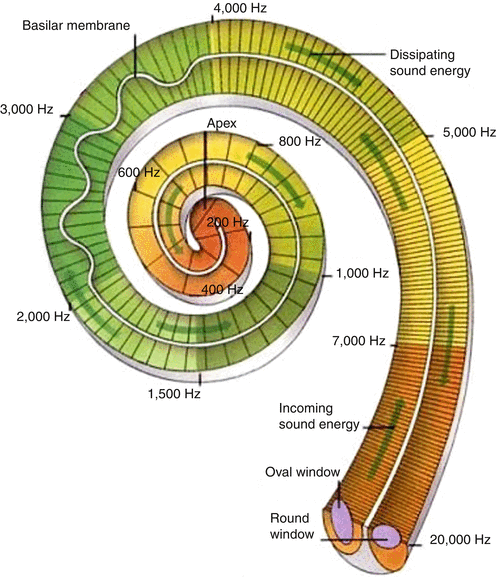
\includegraphics[height=0.6\linewidth]{Imatges_beamer2/coclea.png}
        \caption{Estructura de la còclea \href{https://www.pinterest.com/pin/336995984614355654/}{\enllas}}
        \label{coclea}
    \end{minipage}
    \hfill
    \begin{minipage}[c]{0.49\linewidth}
        \centering
        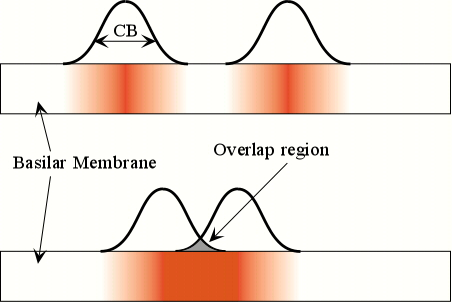
\includegraphics[height=0.6\linewidth]{Imatges_beamer2/basilar_membrane.jpg}
        \caption{Interferència de dos sons en la membrana basilar \href{https://www.phys.uconn.edu/~gibson/Notes/Section7_3/Sec7_3.htm}{\enllas}}
        \label{membrana}
    \end{minipage}
\end{figure}
Això ens porta a concloure que dues freqüències les percebem com a dissonants si es troben dins la mateixa banda i consonants si es troben en bandes diferents. Per tant, és natural preguntar-se quina amplada té aquesta banda crítica, per tal d'estudiar amb més precisió quan dos sons sonen desagradablement.\par
Hi ha diversos models que parametritzen l'amplada de banda crítica corresponent a cada freqüència de l'espectre audible. El més adient pel nostre model és el donat per William Hutchinson i Leon Knopoff en \cite{hutchinson} basat en dades de \cite{plomp,goodwin,mayer} que parametritza l'amplada de banda crítica amb la funció:
\begin{equation}
    \text{CBW}(f)=1.72 f^{0.65}
    \label{CBW}
\end{equation}
Cal mencionar que perquè aquest fórmula tingui sentit (pel que fa a la dimensionalitat) hem de considerar la freqüència $f$ adimensional. Més formalment, en comptes de considerar $f^{0.65}$, es pot considerar una freqüència \textit{normalitzada} per un valor fixat $f_0=1\Hz$, és a dir, considerar ${\left(\frac{f}{f_0}\right)}^{0.65}$. De tota manera, per simplicitat, al llarg del treball utilitzarem la fórmula \eqref{CBW}. D'altra banda, la funció $\text{CBW}(f)$ retorna una amplada mesurada en Hz i, per tant, deduïm que la constant $k=1.72$ té unitats de Hz. D'aquesta manera resolem el problema de la dimensió de $\text{CBW}$.
\section{Model per a la mesura de dissonància}\label{model}
Les demostracions de les proposicions que apareguin en aquesta secció es troben a la secció \ref{demos}.
\subsection{Operacions definides a \texorpdfstring{$\mathcal{C}$}{C}}
Primer de tot, l'objectiu és definir operacions que ens permetin combinar dos (o més) sons complexos en un de sol i modificar la intensitat d'un so complex.
\begin{definition}
    Siguin $\X,\Y\in\mathcal{C}$. Definim la operació \textit{suma $\oplus$} entre sons complexos com l'aplicació:
    \begin{equation*}
        \begin{array}{r@{\hspace{0.5\tabcolsep}}c@{\hspace{0.5\tabcolsep}}c@{\hspace{0.5\tabcolsep}}l}
            \oplus:&\mathcal{C}\times\mathcal{C}&\longrightarrow&\mathcal{C}\\
            &(\X,\Y)&\longmapsto&\X\oplus \Y:=\X\cup\Y
        \end{array}
    \end{equation*}
\end{definition}
\begin{definition}\label{prod_per_escalar}
    Sigui $\lambda\in[0,\infty)$ i $\X=\{(f_1,a_1),(f_2,a_2),\ldots,(f_n,a_n)\}\in\mathcal{C}$. Definim la operació \textit{producte per escalar $\cdot$} entre un so complex i un escalar com l'aplicació:
    \begin{equation*}
        \begin{array}{r@{\hspace{0.5\tabcolsep}}c@{\hspace{0.5\tabcolsep}}c@{\hspace{0.5\tabcolsep}}l}
            \cdot:&\mathcal{C}\times[0,\infty)&\longrightarrow&\mathcal{C}\\
            &(\X,\lambda)&\longmapsto&\lambda\cdot \X:=\Y
        \end{array}
    \end{equation*}
    on $\Y=\{(f_1,\lambda a_1),(f_2,\lambda a_2),\ldots,(f_n,\lambda a_n)\}\in\mathcal{C}$.
\end{definition}
És clar que les operacions $\oplus$ i $\cdot$ sobre el conjunt $\mathcal{C}$ estan ben definides en el sentit que donats dos sons $\X,\Y\in\mathcal{C}$ aleshores $\X\oplus\Y\in\mathcal{C}$ i $\lambda\cdot\X\in\mathcal{C}$. Efectivament, en el primer cas $\X\oplus\Y$ és, per definició, la unió de dos conjunts formats per sons simples, per tant, $\X\oplus\Y$ també serà un conjunt format per sons simples. En el segon cas ja ho hem vist en la pròpia definició.\par
D'altra banda, tot i que aquestes definicions les hem fet entre sons complexos, com que $\mathcal{S}\subset\mathcal{C}$, els sons simples els podem pensar com a sons complexos. Per tant, té sentit també considerar sumes de sons simples i productes de sons simples per escalars, com apareixeran més endavant.
\subsection{Funció de dissonància per a sons simples}
Amb tot això ja podem definir una funció per mesurar el grau de dissonància entre dos sons complexos. Suposem abans de tot que tenim una funció $\delta$ que mesura el grau de dissonància entre dos sons simples. És a dir, $\delta$ és una funció de la forma:
\begin{align*}
    \delta:\mathcal{S}\times\mathcal{S}&\longrightarrow\RR\\
    (s_1,s_2)&\longmapsto\delta(s_1,s_2)
\end{align*}
En aquesta funció li exigim certes propietats que ha de complir:
\begin{enumerate}[label=$\delta$\arabic*),ref=$\delta$\arabic*]
    \item\label{delta1} $\delta(s_1,s_2)=\delta(s_2,s_1)$ per a tot $s_1,s_2\in\mathcal{S}$.
    \item\label{delta2} $\delta(\lambda\cdot s_1,s_2)=\lambda\delta(s_1,s_2)$ per a tot $s_1,s_2\in\mathcal{S}$ i tot $\lambda\in[0,\infty)$.
    \item\label{delta3} $\delta(s_1,\lambda\cdot s_2)=\lambda\delta(s_1,s_2)$ per a tot $s_1,s_2\in\mathcal{S}$ i tot $\lambda\in[0,\infty)$.\par
\end{enumerate}
En aquestes propietats s'entén que, anàlogament a la definició \ref{prod_per_escalar}, si $s_1=(f_1,a_1)$ i $s_2=(f_2,a_2)$, aleshores $\lambda\cdot s_1=(f_1,\lambda a_1)$ i $\lambda\cdot s_2=(f_2,\lambda a_2)$. Aquest fet juntament amb el fet que l'amplitud de qualsevol so és sempre no-negativa, ens fa veure per què $\lambda$ i $\mu$ no poden ser valors negatius. Observem, a més, que la tercera propietat és conseqüència de la primera i la segona. D'altra banda, ajuntant les dues últimes propietats obtenim que $\forall\lambda,\mu\in[0,\infty)$ es compleix $\delta(\lambda\cdot s_1,\mu\cdot s_2)=\lambda\mu\delta(s_1,s_2)$, que és equivalent a dir: $$\delta(s_1,s_2)\propto a_1a_2.$$
\subsection{Model de dissonància per a sons complexos}
L'objectiu ara és crear una funció 
\begin{align*}
    D:\mathcal{C}&\longrightarrow\RR\\
    \X&\longmapsto D(\X)
\end{align*}
que mesuri la dissonància d'un so complex. Per això definirem primer una funció $d$ que mesura la dissonància \textit{relativa} entre dos sons.
\begin{definition}
    Definim la \textit{mesura de la dissonància relativa $d$} entre dos sons complexos com:
    \begin{equation*}
        \begin{array}{r@{\hspace{0.5\tabcolsep}}c@{\hspace{0.5\tabcolsep}}c@{\hspace{0.5\tabcolsep}}l}
            d:&\mathcal{C}\times\mathcal{C}&\longrightarrow&\RR\\
        &(\{s_i\}_{i=1}^n,\{r_i\}_{i=1}^m)&\longmapsto&\frac{1}{2}\sum_{i=1}^n\sum_{j=1}^m\delta(s_i,r_j)
        \end{array}
    \end{equation*}
\end{definition}
\noindent Aquesta funció té les següents propietats:
\begin{prop}\label{prop_dem1}
    Siguin $\X,\Y,\Z\in\mathcal{C}$ sons complexos i $\lambda\in[0,\infty)$. Llavors:
    \begin{enumerate}[label=$d$\arabic*),ref=$d$\arabic*]
        \item\label{d1} $d(\X,\Y)=d(\Y,\X)$.
        \item\label{d2} $d(\X\oplus\Y,\Z)=d(\X,\Z)+d(\Y,\Z)$.
        \item\label{d3} $d(\X,\Y\oplus\Z)=d(\X,\Y)+d(\X,\Z)$.
        \item\label{d4} $d(\lambda\cdot\X,\Y)=\lambda d(\X,\Y)$.
        \item\label{d5} $d(\X,\lambda\cdot\Y)=\lambda d(\X,\Y)$.
    \end{enumerate}
\end{prop}
\noindent Amb aquesta definició, donat un so complex $\X\in\mathcal{C}$, hom pot preguntar-se què ocorre quan avaluem $d(\X,\X)$.
\begin{definition}[Mesura de dissonància]
    Definim la \textit{mesura de la dissonància $D$ d'un so complex} com:
    \begin{align*}
        D:\mathcal{C}&\longrightarrow\RR\\
        \X&\longmapsto d(\X,\X)
    \end{align*}
\end{definition}
\noindent Amb tals definicions obtenim una sèrie de propietats que seran importants a l'hora de calcular la dissonància entre dos (o més) sons de manera computacional \footnote{Per més informació sobre el codi informàtic en llenguatge C veure \url{https://github.com/carlosala/dissonance}.}.
\begin{prop}\label{prop_dem2}
    Siguin $\X,\Y\in\mathcal{C}$ sons complexos i $\lambda\in[0,\infty)$. Llavors:
    \begin{enumerate}[label=$D$\arabic*),ref=$D$\arabic*]
        \item\label{D1} $D(\X\oplus\Y)=D(\X)+D(\Y)+2d(\X,\Y)$.
        \item\label{D2} $D(\lambda\cdot \X)=\lambda^2D(\X)$.
    \end{enumerate}
\end{prop}
\begin{corollary}\label{coro_dem3}
    Siguin $\X_1,\ldots,\X_n\in\mathcal{C}$ sons complexos i $\lambda\in[0,\infty)$ . Aleshores: 
    \begin{equation}\label{eq_final}
        D(\X_1\oplus\cdots\oplus\X_n)=\sum_{i=1}^nD(\X_i)+\sum_{\substack{i,j=1\\i\ne j}}^nd(\X_i,\X_j)=\sum_{i,j=1}^nd(\X_i,\X_j)
    \end{equation}
\end{corollary}
\noindent Observem que la primera d'aquestes últimes propietats (la propietat \ref{D1}) ens permet expressar el valor de $d(\X,\Y)$ en funció únicament de la funció $D$, de la següent manera: $$d(\X,\Y)=\frac{1}{2}\left[D(\X+\Y)-D(\X)-D(\Y)\right].$$
Així doncs aquesta relació juntament amb la de la definició de la funció $D$, $D(\X):=d(\X,\X)$, ens permet passar d'una funció a l'altra i viceversa.\par 
Aquesta estreta relació entre $d$ i $D$, i el fet que ambdues tenen un domini de definició ``similar''\footnote{En aquest cas, el terme ``similar'' fa referència a que un domini està format pel conjunt $\mathcal{C}$ i l'altre pel producte cartesià d'aquest conjunt amb si mateix, és a dir, pel conjunt $\mathcal{C}\times\mathcal{C}$.} ens fa plantejar la possibilitat de ser $d$ una forma bilineal i $D$ la seva forma quadràtica associada. Perquè fos possible això s'hauria de complir que $(\mathcal{C},\oplus,\cdot)$ fos un $\RR$-espai vectorial, que no és cert\footnote{Una manera fàcil de veure que $(\mathcal{C},\oplus,\cdot)$ no és un $\RR$-espai vectorial és tenir en compte que donada una equació de la forma $y(t)=\sum_{i=1}^na_i\sin(2\pi f_it+\varphi_i)$ hi ha més d'un element a $\mathcal{C}$ que la satisfà. En efecte, només cal considerar els sons complexos $\X=\emptyset$ i $\Y=(f,0)$, que són clarament diferents, i satisfan la mateixa equació $y_{\X}(t)=y_{\Y}(t)=0$. Això provoca que, entre altres coses, l'invers d'un element per l'operació $\oplus$ no sigui únic.\newline Si es volgués insistir amb fer un espai vectorial a partir del conjunt $\mathcal{C}$ de sons complexos caldria primer de tot modificar el conjunt de sons simples afegint-hi la fase com a propietat juntament amb la freqüència i amplitud, i d'altra banda també s'hauria de definir una relació $\sim$ de forma que si $\X$ i $\Y$ fossin dos son complexos amb les suposades condicions, aleshores $\X\sim \Y\iff y_{\X}(t)=y_{\Y}(t)$. És fàcil veure que aquesta relació seria d'equivalència. D'aquesta manera es pot veure que el conjunt $\mathfrak{C}$ de les classes d'equivalència juntament amb les operacions $\oplus$ i $\cdot$ retocades convenientment per definir-les sobre $\mathfrak{C}$ (i no sobre $\mathcal{C}$) té estructura de $\RR$-espai vectorial.}. Per tant, $d$ i $D$ són simplement dues aplicacions que satisfan propietats de bilinealitat.
\subsection{Implementació de la funció \texorpdfstring{$\delta$}{delta}} 
Fet aquest plantejament del model de la dissonància, hom pot observar que el valor final depèn única i exclusivament de la funció $\delta$, cosa que intensifica la importància de la seva tria.\par
Per fer-ho, adoptarem un punt de vista biològic: la banda crítica. A més, ens basarem en dades experimentals fetes per Plomp i Levelt \cite{plomp}, cosa que donarà una major credibilitat a la nostra fórmula.\par Com hem explicat a la secció \ref{teoria_auditiva}, quan dues freqüències sonen al mateix instant i s'activen els mateixos nervis de la membrana basilar, diem que les dues freqüències estan en la mateixa banda crítica i, per tant, es produeix interferència, que es tradueix a dissonància. Si les dues freqüències estan suficientment separades en el sentit que s'activen nervis diferents de la membrana basilar, les percebrem com a diferents i, per tant, no hi haurà a penes dissonància entre elles.\par 
Com hem mencionat, per calcular una funció $\delta$ adequada ens hem basat en els estudis empírics de Plomp i Levelt \cite{plomp}. Plomp i Levelt van modelitzar empíricament la dissonància entre dos sons purs. Algunes equacions funcionals que aproximen bé els seus resultats són les següents: $$\delta_1(x)=ae^{-\alpha x}-be^{-\beta x}\qquad\delta_2(x)=\alpha e^{-\left(\log(\beta x)\right)^2}\qquad\delta_3(x)=\beta xe^{-\beta x}$$
Aquestes funcions tenen en comú que, per a valors adequats dels paràmetres, creixen des de 0 fins un valor màxim i a partir d'aquí decreixen de nou fins a zero. Pel nostre model finalment hem decidit adoptar la tercera ja que l'hem vist més apropiada que la segona, i la primera ja ha estat utilitzada per William A. Sethares (veure \cite{sethares1})\footnote{Per altres modelitzacions de corbes de dissonància consultar la feta per David J. Benson \cite{benson} usant també funcions exponencials i la feta per Giorgio Dillon \cite{dillon} usant una funció polinòmica.}. Notem que l'elecció de la funció usada no és una cosa objectiva, degut a la falta de precisió de les dades de Plomp i Levelt i la subjectivitat de la percepció de la dissonància. L'objectiu principal que ha de satisfer la funció, més enllà de les propietats \ref{delta1}-\ref{delta3}, és que tingui unes característiques que s'ajustin bé als resultats empírics \cite{benson}.\par
Així doncs, donats dos sons simples $s_1=(f_1,a_1)$ i $s_2=(f_2,a_2$, volem calcular una funció de dissonància $\delta(s_1,s_2)$. Com hem mencionat, per crear aquesta funció tindrem en compte el concepte de banda crítica, introduïa a la secció \ref{teoria_auditiva}. Segons dades de E. Zwicker, G. Flottorp i S. S. Stevens \cite{zwicker} la màxima dissonància entre els sons $s_1$ i $s_2$ es troba quan les seves respectives freqüències ($f_1$ i $f_2$) estan separades aproximadament un 25\% de l'amplada de la banda crítica de la freqüència mitjana $f_m:=\frac{f_1+f_2}{2}$. És a dir, les freqüències $f_1$ i $f_2$ tindran una dissonància màxima quan $\frac{|f_1-f_2|}{\text{CBW}(f_m)}=0.25$. Així doncs, per determinar el valor de $\beta$ (que dependrà de $f_1$ i $f_2$) de la funció $\beta xe^{-\beta x}$ hem de tenir en compte que s'ha d'assolir el màxim en la freqüència esmentada. Tenim doncs que:
$$\left(\beta xe^{-\beta x}\right)'=0\iff \beta e^{-\beta x}(1-\beta x)=0\iff\beta x=1.$$ A més com que $$\left(\beta xe^{-\beta x}\right)''=\beta^2e^{-\beta x}(\beta x-2),$$ efectivament tenim un màxim quan $\beta x=1$.
En el cas que ens ocupa, prenem $x=\frac{|f_2-f_1|}{\min(f_1,f_2)}$. És a dir, prenem $x$ com la resta de les dues freqüències normalitzada. Com que sabem que el màxim s'assoleix quan $\frac{|f_1-f_2|}{\text{CBW}(f_m)}=0.25$ tindrem que:
$$\frac{|f_1-f_2|}{\text{CBW}(f_m)}=0.25\iff\frac{\min(f_1, f_2)}{\text{CBW}(f_m)\cdot 0.25}\cdot\frac{|f_1-f_2|}{\min(f_1, f_2)}=1=\beta x\iff\beta=\beta(f_1,f_2)=\frac{\min(f_1, f_2)}{\text{CBW}(f_m)\cdot 0.25}.$$
Així doncs per a la funció de dissonància sabem que: $$\delta(s_1,s_2)=\delta((f_1,a_1),(f_2,a_2))\propto\beta(f_1,f_2)xe^{-\beta(f_1,f_2)x}$$ Recordant dues de les propietats necessàries (\ref{delta2} i \ref{delta3}) que ha de complir la funció $\delta$ deduïm que: $$\delta((f_1,a_1),(f_2,a_2))\propto a_1a_2.$$ Finalment la nostra funció de dissonància $\delta$ triada és: $$\delta((f_1,a_1),(f_2,a_2))=a_1a_2\beta(f_1,f_2)\frac{|f_2-f_1|}{\min(f_1,f_2)}e^{-\beta(f_1,f_2)\frac{|f_2-f_1|}{\min(f_1,f_2)}}$$
O, equivalentment, si simplifiquem l'expressió i l'escalem de tal forma que la màxima dissonància valgui 1 quan les amplituds valguin 1, obtenim: 
\begin{equation}
    \delta((f_1,a_1),(f_2,a_2))=a_1a_2\frac{|f_2-f_1|}{\text{CBW}(f_m)\cdot 0.25}e^{1-\frac{|f_2-f_1|}{\text{CBW}(f_m)\cdot 0.25}}
    \label{for:dissonancia}
\end{equation}
Observem que, pel comentaris fets prèviament en les seccions \ref{teoria_musical} i \ref{teoria_auditiva}, la funció $\delta$ no té unitats. A la figura \ref{main:fig3} es mostra un exemple gràfic d'aquesta fórmula per a diferents sons purs.
\begin{center}
    \includestandalone[mode=image|tex,width=0.5\linewidth]{Imatges_main/model2}
    \captionof{figure}{Representació de la funció $\delta(s_1,s_2)$, on $s_1=(f_1,1)$ i $s_2=(f_2,1)$ a partir de varies freqüències fixades $f_1$ i fent variar $f_2$ o, més ben dit, fent variar $\frac{f_2}{f_1}$ suposant $f_2\geq f_1$.}
    \label{main:fig3}
\end{center}
\subsection{Anàlisi dels resultats}
Amb la implementació de la funció $\delta$ en l'apartat anterior ara ja podem treure les primeres conclusions. Per això, construïm ara un exemple d'aplicació d'aquesta model.\par Suposem que estem treballant amb sons complexos que són notes musicals, és a dir, amb conjunts de sons simples les freqüències dels quals són múltiples enters de una freqüència fonamental. Suposem a més que l'amplitud de l'harmònic $k$-èssim és $1/k^\alpha$, on $\alpha\in\mathbb{R}$ és un paràmetre fixat arbitrari. És a dir, la freqüència fonamental té amplitud 1, el segon harmònic té amplitud $1/2^\alpha$; el tercer, $1/3^\alpha$... Si fixem una nota musical $\N_1$ (de freqüència fonamental $f_1$) i fem variar-ne una altra $\N_2$ (de freqüència fonamental $f_2$) a partir d'un índex $r\in[1,2]$ tal que $f_2=rf_1$, obtenim els resultats que es mostren a les figures següents. Cal mencionar que en el nostre treball hem agafat $\alpha=0,75$. A més, en les imatges que hi ha a continuació han estat fetes considerant 9 harmònics de cada nota musical. Això últim ho he fet a causa del ràpid decreixement dels harmònics a partir del 10 i la tria $\alpha$ ha estat feta de manera que l'amplitud dels 9 primers harmònics s'aproximés relativament bé. A la següent imatge es mostre el comportament d'aquests harmònics.\par
\begin{figure}[ht]
    \centering
    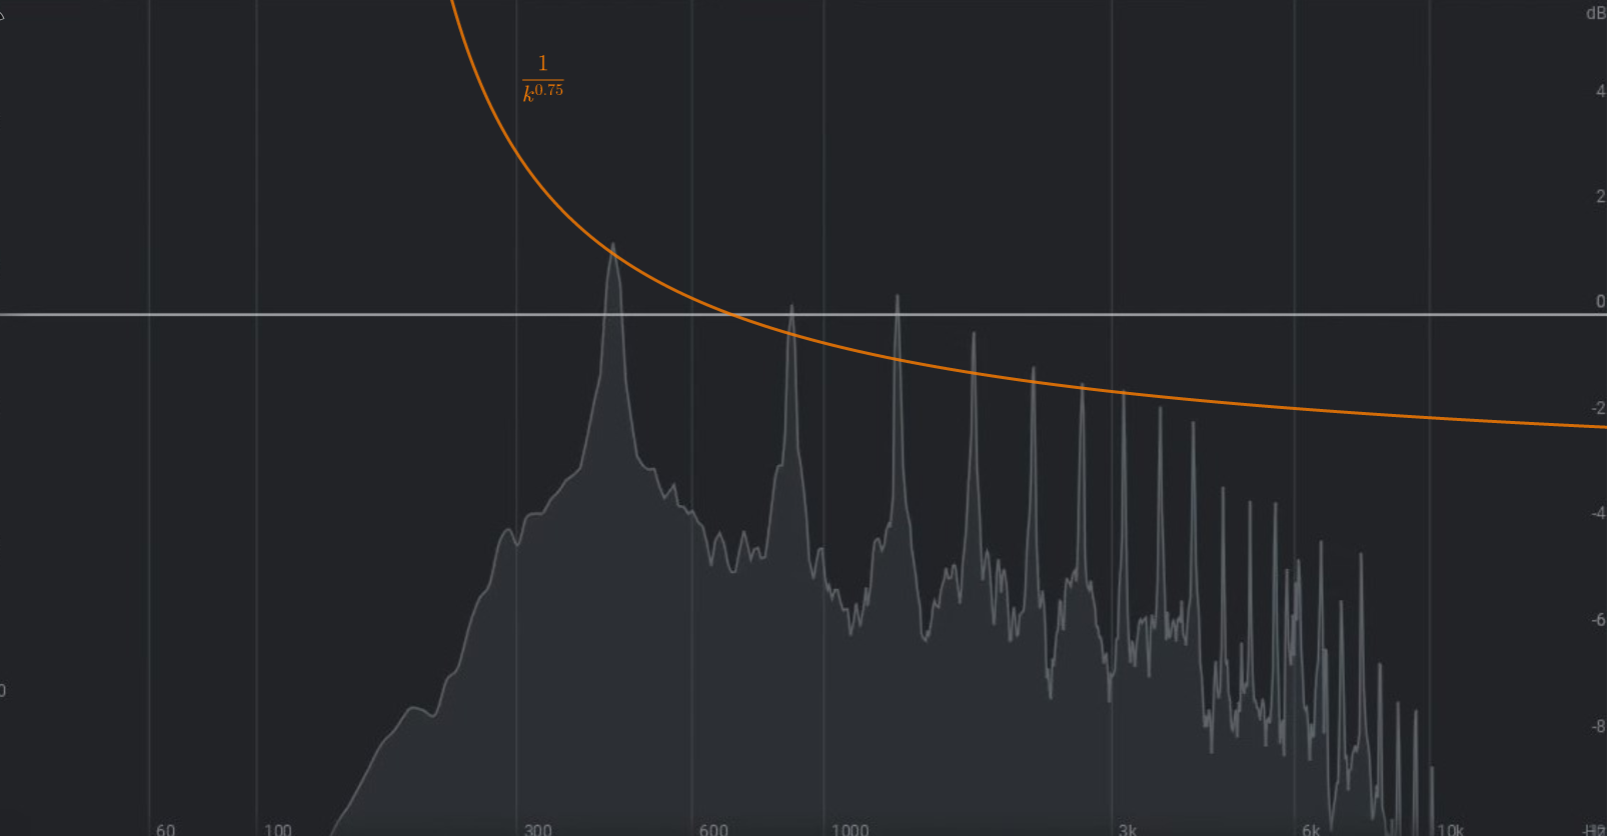
\includegraphics[width=0.5\linewidth]{Imatges_main/espectre_freq.png}
    \caption{Representació de l'espectre de freqüències de la nota LA4 (440 Hz) juntament amb la funció $\frac{1}{k^{0.75}}$ aproximant l'amplitud dels primers 9 harmònics}
\end{figure}
En els següents gràfics podem observar les \textit{corbes de dissonància} creades a partir del model descrit anteriorment.
\begin{center}
    \includestandalone[mode=image|tex,width=0.49\linewidth]{Imatges_main/complex1}
    \includestandalone[mode=image|tex,width=0.49\linewidth]{Imatges_main/complex2}\\
    \includestandalone[mode=image|tex,width=0.49\linewidth]{Imatges_main/complex3}
    \captionof{figure}{Dissonància entre dos notes musicals $\N_1$ i $\N_2$. Aquí hem fixat la freqüència fonamental de $\N_1$ a 100 Hz, 440 Hz i 1760 Hz, respectivament i hem fet variar la relació $f_2/f_1$, essent $f_2$ la freqüència fonamental de $\N_2$.}
    \label{fig:complex}
\end{center}
Observem la peculiar forma dels gràfics. En particular sembla que se satisfà que els punts de màxima consonància es troben quan el quocient de les dues freqüències fonamentals de les notes $\N_1$ i $\N_2$ és una fracció involucrant nombres enters senzills en el numerador i denominador, tal com ja teoritzaven el pitagòrics al segle \MakeUppercase{\romannumeral 6} aC. Això es deu al següent fet: considerem notes musicals $\N_1$ i $\N_2$ amb freqüències fonamentals $f_1$ i $f_2$, respectivament, tals que $\frac{f_2}{f_1}=\frac{p}{q}$, on $p,q\in\NN$ són nombres enters positius i coprimers. És a dir, $pf_1=qf_2$. Això vol dir que la freqüència de l'harmònic $p$-èssim de $f_1$ serà la mateix que la de l'harmònic $q$-èssim de $f_2$, i com a conseqüència $\delta((pf_1,a_1),(qf_2,a_2))=0$, per la definició de la funció $\delta$. De fet, això últim ocorrerà sempre que es comparin dos sons simples de freqüències $kpf_1$ i $kqf_2$, $k\in\NN$. Això comporta que si els valors de $p$ i $q$ són petits, aquestes igualtats entre harmònics s'aniran repetint constantment, el que provocarà un no-creixement en el valor total de la dissonància de $\N_1\oplus\N_2$. En canvi, si $p$ i $q$ són valors grans, la igualtat entre els harmònics ocorrerà quan n'haguem considerat molts i, per tant, a cada sumand de l'equació \eqref{eq_final} sempre anirem aportant petites (però no nu\lgem es) contribucions en la dissonància total, el que provoca que al final de tot el valor de $D(\N_1\oplus\N_2)$ sigui més gran.\par D'altra banda, notem que conforme augmentem la freqüència base $f_1$ la dissonància en general va disminuint. Això és degut a la forma de la funció $\delta$ i també del comportament de la funció $\text{CBW}$ a freqüències altes. Aquest fet explica el per què no se sol produir música amb notes musicals que tenen freqüències fonamentals menors a 100 Hz.\par Fet aquest anàlisis i havent vist que en general la funció dissonància perd magnitud a mesura que considerem sons més aguts, si $\N_1$ i $\N_2$ són dos sons amb freqüències fonamentals $f_1$ i $f_2$, un pot preguntar-se què ocorre quan fixem una fracció $\frac{p}{q}$, on $p,q\in\NN$, i considerem que el quocient de freqüències $\frac{f_1}{f_2}$ sigui igual a $\frac{p}{q}$. És a dir quina dissonància percebem quan fixem $\frac{f_2}{f_1}=\frac{p}{q}$. És clar que la dissonància $D(\N_1\oplus\N_2)$ resultat d'haver combinat aquests dos sons amb la relació de freqüències mencionada variarà de forma decreixent. Per tal de representar gràficament i poder percebre amb més claredat com és aquest decreixement, al següent gràfic hem representat quatre fraccions $\frac{p}{q}$ i hem fet variar $f_1$ en l'interval $[60,1000]$.
\begin{figure}[ht]
    \centering
    \includestandalone[mode=image|tex,width=0.6\linewidth]{Imatges_main/grafic_fraccio_pq}
    \caption{Variació de la dissonància de les notes musicals $\N_1$ i $\N_2$ amb respectives freqüències fonamentals $f_1$ i $f_2$, imposant que $\frac{f_2}{f_1}=\frac{p}{q}$, per a diferents fraccions $\frac{p}{q}$.}
\end{figure}
\section{Anàlisi dels fets empírics}
Per comprovar que el model és encertat, vam realitzar un test a una mostra d'aproximadament 200 persones. El test consistia en 11 sons diferents, 3 corresponents a combinacions de freqüències baixes $(f \approx 110\Hz)$, 4 corresponents a freqüències mitjanes $(f \approx 440\Hz)$ i 4 corresponents a freqüències altes $(f \approx 1760\Hz)$. L'oient havia qualificar-los amb un número de l'1 al 10, essent 1 el nivell més dissonant i 10 el menys dissonant. El test també demanava a l'enquestat l'edat i, més important encara, la seva formació musical, que podia variar entre 5 nivells diferents (molt baix, baix, intermedi, alt i molt alt). Per tal de verificar que la gent era honesta amb la seva puntuació sobre el nivell de formació musical vam demanar, a més, que descrivissin breument la seva trajectòria musical. \par
En total vam aconseguir 190 respostes, de les quals 42 eren de nivell molt baix; 69, de nivell baix; 43, de nivell intermedi; 26, de nivell alt, i 10, de nivell alt. Aquesta separació entre grups ens va permetre poder classificar les dades en 3 grups segons el nivell de formació musical: nivell molt baix-baix (111 respostes), nivell intermedi (43 respostes) i nivell alt-molt alt (36 respostes). \par
Al test únicament vam incloure combinacions de dos notes $\N_1$ i $\N_2$ de l'escala musical d'un piano. Pel primer d'ells vam elegir sempre la nota LA de freqüències 110 Hz, 440 Hz i 1760 Hz, respectivament segons el rang de freqüències (baixes, mitjanes o altes) que estiguéssim treballant. A continuació veiem la freqüència (i la seva nota corresponent) amb que vam combinar aquestes notes i quin hauria de ser el resultat obtingut segons el nostre model:
\begin{table}[ht]
    \centering
    \begin{tabular}{| c | c | c | c |}
    \cline{2-4}
    \multicolumn{1}{c|}{} & $\N_1$ & $\N_2$ & $D(\N_1\oplus\N_2)$\\
    \hline
    \hline
    So 1 & \multirow{3}{2.5cm}{LA2 $(110\Hz)$} & SI2 $(123.47\Hz)$ & 2.1409\\
    \cline{1-1}\cline{3-4}
    So 2 & & MI3 $(164.81\Hz)$ & 0.7900\\		
    \cline{1-1}\cline{3-4}
    So 3 & & SOL3 $(196\Hz)$  & 1.2839\\
    \hline
    So 4 & \multirow{4}{2.5cm}{LA4 $(440\Hz)$} & LA\#4 $(466.16\Hz)$ & 1.8835 \\
    \cline{1-1}\cline{3-4}
    So 5 & & RE5 $(587.33\Hz)$  & 0.3891 \\
    \cline{1-1}\cline{3-4}
    So 6 & & RE\#5 $(622.25\Hz)$ & 0.6032 \\
    \cline{1-1}\cline{3-4}
    So 7 & & FA5 $(698.46\Hz)$ & 0.5752 \\
    \hline
    So 8 & \multirow{4}{2.5cm}{LA6 $(1760\Hz)$} & LA\#6 $(1864.66\Hz)$ & 1.2451 \\
    \cline{1-1}\cline{3-4}
    So 9 & & DO\#7 $(2217.46\Hz)$ & 0.2617 \\
    \cline{1-1}\cline{3-4}
    So 10 & & MI7 $(2637.02\Hz)$ & 0.09559 \\
    \cline{1-1}\cline{3-4}
    So 11 & & FA\#7 $(2959.96\Hz)$ & 0.2156 \\
    \hline
    \end{tabular}
    \caption{Freqüències usades al test i dissonància predita pel nostre model}
    \label{tab:3}
\end{table}\par
Els següents gràfics mostren de manera més clara on se situen les combinacions de notes escollides pel que fa a la dissonància entre elles:
\begin{center}
    \includestandalone[mode=image|tex,width=0.49\linewidth]{Imatges_main/complex1_marcat}
    \includestandalone[mode=image|tex,width=0.49\linewidth]{Imatges_main/complex2_marcat}\\
    \includestandalone[mode=image|tex,width=0.49\linewidth]{Imatges_main/complex3_marcat}
    \captionof{figure}{Gràfic on es mostra la posició de les combinacions de sons escollides pel test en les corbes de dissonància}
\end{center}
Els següent gràfic mostra els resultats obtinguts en el test.\par
\begin{figure}[ht]
    \centering
    \includestandalone[mode=image|tex,width=0.6\linewidth]{Imatges_main/mediana}
    \caption{Resultats del test juntament amb la predicció (reescalada convenientment) dels nostres resultats}
\end{figure}
Per a l'anàlisi dels resultats ens hem basat en la mediana dels tots els valors obtinguts. El motiu de no haver inclòs la mitjana o la moda juntament amb la mediana es deu al fet que la primera està molt condicionada pels valors centrals de manera que les puntuacions mitjanes de cada so eren totes relativament similar, i no haurien de ser-ho per l'elecció feta dels sons. Pel que fa a la moda, aquesta ens va condicionar molt els valors extrems ja que molta gent puntuava la dissonància dels sons amb valors molt radicals: o propers a 1, o propers a 10.\par
Observem que hi ha clares diferències entre els diferents nivells. En particular, deduïm que quan més familiar ens és un so, millor són els resultats predits pel model. Efectivament, en els sons 4, 5, 6 i 7, que són els de freqüències mitjanes (i.e. els més comuns), l'error comès en l'aproximació teòrica és inferior en comparació amb l'aproximació del model dels sons greus (sons 1, 2 i 3) i els sons aguts (sons 8, 9, 10 i 11). Podem concloure, doncs, que els resultats empírics obtinguts verifiquen prou bé els resultats obtinguts al nostre model.\par Finalment, cal comentar també que, tot i haver-ho considerat, al final no vam fer cap distinció per rangs d'edat. Això ho vam decidir així perquè no vam posar sons extremadament greus (el mínim va ser d'aproximadament 100 Hz) ni extremadament aguts (el màxim va ser d'aproximadament 3000 Hz), que són els que es deixen d'escoltar abans. Això juntament amb el fet que va haver molt pocs enquestats de més de 60 anys (que és quan l'oïda comença a deteriorar-se substancialment) en comparació amb el resta de rangs d'edat, ens va fer descartar aquesta possibilitat.
\section{Conclusions i possibles refinaments}
Malgrat ser aquest tema de la dissonància molt subjectiu, al llarg del treball hem vist que és possible modelar la dissonància partint de fenòmens auditius com és el de la banda crítica.\par
Una possible extensió és endinsar-nos més en l'estructura algebraica que hi ha darrera el conjunt de sons complexos. Per això caldria, però, redefinir el conjunt de sons simples i incorporar-li un nou factor: la fase del so. Això ens permetria, juntament amb petites modificacions, definir les funcions $d$ i $D$ sobre un espai vectorial de dimensió infinita\footnote{De fet, seria no només infinit el conjunt, sinó no numerable.}. D'aquesta manera $d$ seria una forma bilineal i $D$ la seva forma quadràtica associada, ambdues sobre l'espai vectorial en qüestió.\par
Referent al test, degut a la situació de la pandèmia no vam poder dur-lo a terme amb les condicions idònies que haguéssim volgut. La forma ideal de fer aquest test hagués estat assegurar-nos que tothom escoltés els sons amb els mateixos auriculars i en un ambient silenciós, per tal d'eliminar possibles factors externs interferint en els resultats.\par
També enfocat a una millora del test, podríem haver experimentat amb combinacions de tres o quatre notes musicals tocades simultàniament, que de fet són les que solem sentir quan escoltem una melodia d'un piano, per exemple. \par Para\lgem elament a aquest darrer tema, també podríem haver considerat la possibilitat d'incloure diversos instruments i fer un estudi de com varia la percepció de la dissonància segons la classe d'instrument (de vent, de corda, de percussió...) que estiguem considerant, amb l'objectiu de descobrir quin d'ells és aproximat més satisfactòriament pel nostre model.
\section{Agraïments}
Primer de tot agraïm a la Natàlia Castellana Vila, tutora del treball, per la seva exigència i el constant suport al llarg de tot el projecte. \par
D'altra banda, agraïm també al professor de l'assignatura, Xavier Mora Giné, per l'increïble implicació en aquest treball així com la participació en el debat de qüestions formals del treball.\par 
Finalment, i no menys important, també volem deixar constància de tots aquells professors de l'assignatura que han aportat i compartit les seves crítiques i idees amb el propòsit de millorar i consolidar el treball.
\printbibliography[heading=bibintoc]
\appendix
\section{Demostracions}\label{demos}
\begin{prop*}[\ref*{prop_dem1}]
    Siguin $\X,\Y,\Z\in\mathcal{C}$ sons complexos i $\lambda\in[0,\infty)$. Llavors:
    \begin{enumerate}[label=$d$\arabic*),ref=$d$\arabic*]
        \item\label{dd1} $d(\X,\Y)=d(\Y,\X)$.
        \item\label{dd2} $d(\X\oplus\Y,\Z)=d(\X,\Z)+d(\Y,\Z)$.
        \item\label{dd3} $d(\X,\Y\oplus\Z)=d(\X,\Y)+d(\X,\Z)$.
        \item\label{dd4} $d(\lambda\cdot\X,\Y)=\lambda d(\X,\Y)$.
        \item\label{dd5} $d(\X,\lambda\cdot\Y)=\lambda d(\X,\Y)$.
    \end{enumerate}
\end{prop*}
\begin{proof}
    Suposem que $\X=\{x_i\}_{i=1}^n$, $\Y=\{y_i\}_{i=1}^m$ i $\Z=\{z_i\}_{i=1}^p$.
    \begin{enumerate}[label=$d$\arabic*)]
        \item $$d(\X,\Y)=\frac{1}{2}\sum_{i=1}^n\sum_{j=1}^m\delta(x_i,y_j)=\frac{1}{2}\sum_{j=1}^m\sum_{i=1}^n\delta(y_j,x_i)=d(\Y,\X),$$ on hem utilitzat que la funció $\delta$ és simètrica (propietat \ref{delta1}).
        \item Per simplificar la notació, anomenem 
        $$
        w_i=\left\{
        \begin{array}{ccc}
            x_i & \text{si} & 1\leq i\leq n\\
            y_{i-n} & \text{si} & n+1\leq i\leq m
        \end{array}\right.
        $$ Aleshores tenim que: $$d(\X\oplus\Y,\Z)=\frac{1}{2}\sum_{i=1}^{n+m}\sum_{j=1}^p\delta(w_i,z_j)=\frac{1}{2}\sum_{i=1}^n\sum_{j=1}^p\delta(x_i,z_j)+\frac{1}{2}\sum_{i=n+1}^m\sum_{j=1}^p\delta(y_i,z_j)=d(\X,\Z)+d(\Y,\Z).$$
        \item És conseqüència de les propietats \ref{dd1} i \ref{dd2}.
        \item $$d(\lambda\cdot\X,\Y)=\frac{1}{2}\sum_{i=1}^n\sum_{j=1}^m\delta(\lambda x_i,y_j)=\frac{\lambda}{2}\sum_{i=1}^n\sum_{j=1}^m\delta(x_i,y_j)=\lambda d(\X,\Y),$$ on hem aplicat la propietat \ref{delta2}.
        \item És conseqüència de les propietats \ref{dd1} i \ref{dd4}.
    \end{enumerate}
\end{proof}
\begin{prop*}[\ref*{prop_dem2}]
    Siguin $\X,\Y\in\mathcal{C}$ sons complexos i $\lambda\in[0,\infty)$. Llavors:
    \begin{enumerate}[label=$D$\arabic*),ref=$D$\arabic*]
        \item\label{DD1} $D(\X\oplus\Y)=D(\X)+D(\Y)+2d(\X,\Y)$.
        \item\label{DD2} $D(\lambda\cdot \X)=\lambda^2D(\X)$.
    \end{enumerate}
\end{prop*}
\begin{proof}
    \hfill
    \begin{enumerate}[label=$D$\arabic*)]
        \item Aplicant les propietats \ref{dd1}, \ref{dd2} i \ref{dd3} obtenim:
        \begin{multline*}
            D(\X\oplus\Y)=d(\X\oplus\Y,\X\oplus\Y)=d(\X,\X\oplus\Y)+d(\Y,\X\oplus\Y)=d(\X,\X)+d(\X,\Y)+\\+d(\Y,\X)+d(\Y,\Y)=d(\X,\X)+d(\Y,\Y)+2d(\X,\Y)=D(\X)+D(\Y)+2d(\X,\Y).
        \end{multline*}
        \item Aplicant les propietats \ref{dd4} i \ref{dd5} obtenim: $$D(\lambda\cdot\X)=d(\lambda\cdot\X,\lambda\cdot\X)=\lambda d(\X,\lambda\cdot\X)=\lambda^2d(\X,\X)=\lambda^2D(\X).$$
    \end{enumerate}
\end{proof}
\begin{corollary*}[\ref*{coro_dem3}]
    Siguin $\X_1,\ldots,\X_n\in\mathcal{C}$ sons complexos i $\lambda\in[0,\infty)$. Aleshores: $$D(\X_1\oplus\cdots\oplus\X_n)=\sum_{i=1}^nD(\X_i)+\sum_{\substack{i,j=1\\i\ne j}}^nd(\X_i,\X_j)=\sum_{i,j=1}^nd(\X_i,\X_j)$$
\end{corollary*}
\begin{proof}
    Ho demostrarem per inducció sobre $n$. Per $n=1$ clarament es compleix la igualtat.\par 
    \noindent Suposem certa la igualtat per $n=k$ i demostrem-la per $n=k+1$. Per les propietats \ref{DD1} i \ref{dd2} tenim que:
    \begin{multline*}
        D(\X_1\oplus\cdots\oplus\X_{k+1})=D([\X_1\oplus\cdots\oplus\X_k]\oplus\X_{k+1})=D(\X_1\oplus\cdots\oplus\X_k)+\\+D(\X_{k+1})+2d(\X_1\oplus\cdots\oplus\X_k,\X_{k+1})=D(\X_1\oplus\cdots\oplus\X_k)+D(\X_{k+1})+2\sum_{i=1}^kd(\X_i,\X_{k+1}).
    \end{multline*}
    Ara bé, per la hipòtesi d'inducció tenim que:
    $$D(\X_1\oplus\cdots\oplus\X_k)=\sum_{i=1}^kD(\X_i)+\sum_{\substack{i,j=1\\i\ne j}}^kd(\X_i,\X_j).$$ Així doncs, ajuntant-ho tot obtenim:
    \begin{multline*}
        D(\X_1\oplus\cdots\oplus\X_{k+1})=\sum_{i=1}^kD(\X_i)+\sum_{\substack{i,j=1\\i\ne j}}^kd(\X_i,\X_j)+D(\X_{k+1})+2\sum_{i=1}^kd(\X_i,\X_{k+1})=\\=\sum_{i=1}^{k+1}D(\X_i)+\sum_{\substack{i,j=1\\i\ne j}}^{k+1}d(\X_i,\X_j).
    \end{multline*}
    Finalment, si expressem en aquesta igualtat $D(\X_i)$ com $d(\X_i,\X_i)$ deduïm la segona igualtat del coro\lgem ari.
\end{proof}
\end{document}
